\documentclass{article}

% (fold)
\usepackage{booktabs,amsmath} 
\newcommand{\dpder}[3][]{\dfrac{\partial^{#1}#2}{\partial #3}} \addtolength{\oddsidemargin}{-.875in} \addtolength{\evensidemargin}{-.875in} \addtolength{\textwidth}{1.75in}

\addtolength{\topmargin}{-.875in} \addtolength{\textheight}{1.75in}

% need for subequations
\usepackage{graphicx} 

% need for figures
\usepackage{verbatim} 

% useful for program l,istings
\usepackage{color} 

% use if color is used in text
\usepackage{subfigure}

% use for side-by-side figures
\usepackage[pdfpagemode={UseOutlines},bookmarks=true,bookmarksopen=true, bookmarksopenlevel=0,bookmarksnumbered=true,hypertexnames=false, colorlinks,linkcolor={blue},citecolor={blue},urlcolor={red}, pdfstartview={FitV},unicode,breaklinks=true]{hyperref} 

% use for hypertext links, including those to external documents and URLs
\newcommand{\minus}{\scalebox{0.75}[1.0]{$-$}}
\newcommand{\ajp}{AJP} 
\newcommand{\ig}{ 
\includegraphics} 
\newcommand{\tu}{\textup} \hypersetup{urlcolor=blue, colorlinks=true} 
\sloppy
\definecolor{lightgray}{gray}{0.5}
\setlength{\parindent}{0pt}
% Colors hyperlinks in blue - change to black if annoying
% don't need the following. simply use defaults
\setlength{\baselineskip}{16.0pt} 

% 16 pt usual spacing between lines
\begin{comment}
	\pagestyle{empty} 
	
	% use if page numbers not wanted
\end{comment}

% Specifies the directory where pictures are stored
% above is the preamble (end)
\begin{document} 
\title{Homework 1: Heat Equation} 
\author{DN2255 \\ Kevin Mead}

%\affiliation{KTH Royal Institute of Technology, Electrotechnical Modelling} \email{kmead@kth.se}
\date{\today} 
\maketitle 


%!TEX root = /Users/kevin/SkyDrive/KTH Work/LaTeX Reports/Heat Equation/Heat Equation.tex
\section{Heat Equation} 

% (fold)
\label{sec:heat_equation}
\begin{align}
	& q_t = \nabla \cdot (\nabla q) + S \label{eq:equation1} \\
	& q(x,y,0) = 0 \label{eq:equation2} \\
	& \mathbf{n} \cdot \nabla q = 0 \label{eq:equation3}
\end{align}

\subsection{Analytical preamble} % (fold)
\label{sub:analytical_preamble}
\begin{enumerate}
	\item Flux vector from (\ref{eq:equation1}), $\vec{F}=-\nabla q$
	\item Determine $Q(t) = \int_{0}^{1} \int_{0}^{1} q(x,y,t)dxdy$
\end{enumerate}
% subsection analytical_preamble (end)
% section heat_equation (end)

%!TEX root = /Users/kevin/SkyDrive/KTH Work/Period 3 2014/DN2255/Homework/1/Heat Equation/Heat Equation.tex
\section{Discretization and implementation} 

% (fold)
\label{sec:discretization_and_implementation} 
\begin{figure}[htbp] 
	\centering 
	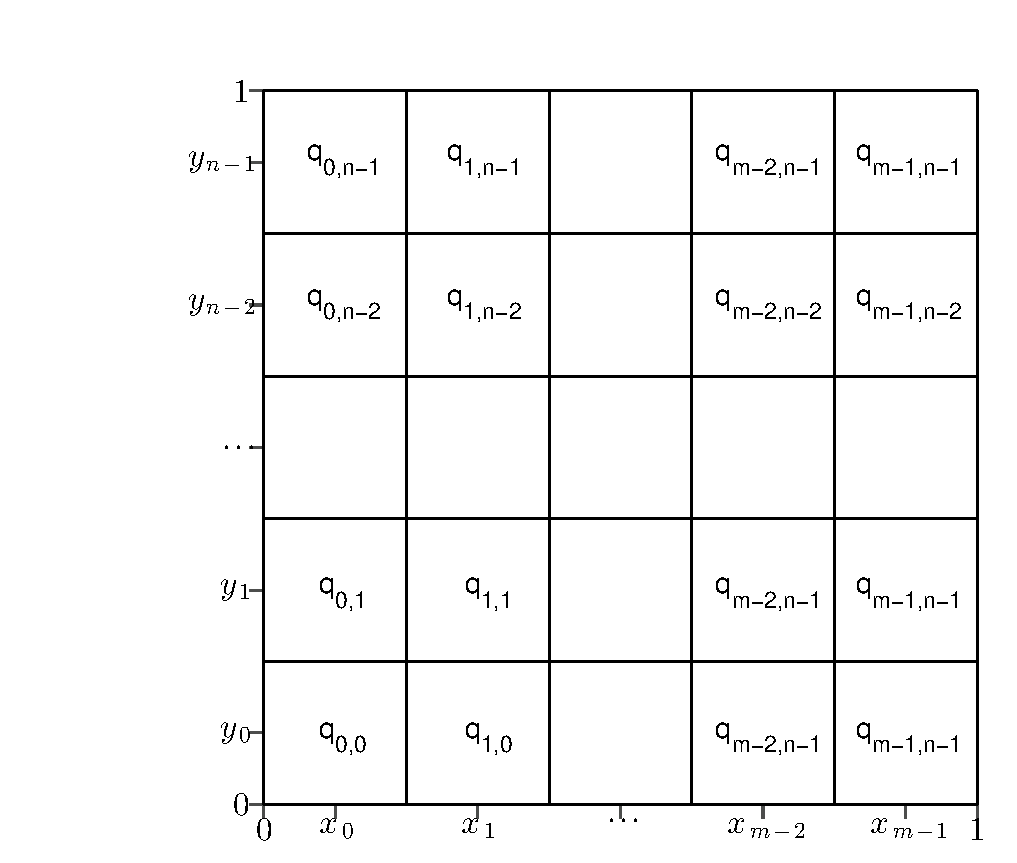
\includegraphics[width=.7\textwidth]{Figures/gridForNumericalSchemePlot.eps} \caption{Finite volume grid} \label{fig:Figures_gridForNumericalSchemePlot} 
\end{figure}

Let $Q_{ij}$ denote the cell average of q over cell (i,j) so, 
\begin{equation}
	Q_{ij}(t) = \frac{1}{\Delta x \Delta y} \int_{x_{i-1/2}}^{x_{i+1/2}}\int_{y_{j-1/2}}^{y_{j+1/2}} q(x_i,y_j,t) dxdy \label{eq:qCellAverage} 
\end{equation}
and defining $S_{ij}$ as the cell average of S over cell (i,j), 
\begin{equation}
	S_{ij}(t) = \frac{1}{\Delta x \Delta y} \int_{x_{i-1/2}}^{x_{i+1/2}}\int_{y_{j-1/2}}^{y_{j+1/2}} S(x_i,y_j,t) dxdy \label{eq:sCellAverage} 
\end{equation}
where $\Delta x = x_{i+1/2}-x_{i-1/2}$ and $\Delta y = y_{j+1/2}-y_{j-1/2}$ 
\begin{enumerate}
	\item Derive a finite volume method for the spatial part of (\ref{eq:equation1}) by integrating and forming cell averages. 
	\begin{align*}
		& q_t = \nabla \cdot (\nabla q) + S \\
		& \iint \limits_{\Delta x \, \Delta y} q_t = \iint \limits_{\Delta x \, \Delta y} \nabla^2 q + \iint \limits_{\Delta x \, \Delta y} S \\
		& \frac{d}{dt} \iint \limits_{\Delta x \, \Delta y} q = \iint \limits_{\Delta x \, \Delta y} \left( \frac{d^2 q}{dx^2} + \frac{d^2 q}{dy^2} \right) + \iint \limits_{\Delta x \, \Delta y} S 
	\end{align*}
	and now dividing everything by the common cell area $\Delta x \Delta y$, we can use (\ref{eq:qCellAverage}) and (\ref{eq:sCellAverage}) to get 
	\begin{align}
		& \frac{d}{dt} Q_{ij}(t) = \frac{1}{\Delta x \Delta y}\iint \limits_{\Delta x \, \Delta y} \left( \frac{d^2 q}{dx^2} + \frac{d^2 q}{dy^2} \right) + S_{ij}(t) \label{eq:eqCommon} 
	\end{align}
	
	I will Taylor expansions to define the Laplacian terms. The Taylor expansions of $q(x_i+\Delta x)$ and $q(x_i-\Delta x)$, taking the derivative with respect to x are
	
	% \begin{align*}
	% 	& q(x_i+\Delta x) = q(x_i) + \Delta x \, q'(x_i) + \frac{1}{2} (\Delta x)^2 q''(x_i) + \frac{1}{6} (\Delta x)^3 q'''(\zeta_+) \\
	% 	& q(x_i-\Delta x) = q(x_i) - \Delta x \, q'(x_i) + \frac{1}{2} (\Delta x)^2 q''(x_i) - \frac{1}{6} (\Delta x)^3 q'''(\zeta_-) 
	% \end{align*}
	\begin{align}
		& q(x_i+\Delta x) = q(x_i) + \Delta x \, q'(x_i) + \frac{1}{2} (\Delta x)^2 q''(x_i) + \frac{1}{6} (\Delta x)^3 q'''(x_i) + \frac{1}{24} (\Delta x)^4 q^{(4)}(\zeta_+) \label{eq:taylorExp1}\\
		& q(x_i-\Delta x) = q(x_i) - \Delta x \, q'(x_i) + \frac{1}{2} (\Delta x)^2 q''(x_i) - \frac{1}{6} (\Delta x)^3 q'''(x_i) + \frac{1}{24} (\Delta x)^4 q^{(4)}(\zeta_-) \label{eq:taylorExp2} 
	\end{align}
	where the last terms represent a value $\zeta_\pm$ that makes the truncation of the Taylor expansion exactly equal to the infinite series. Since we do not know this value, we must remove it and it will be our truncation error. Adding (\ref{eq:taylorExp1}) with (\ref{eq:taylorExp2}) and rearranging terms, 
	\begin{align*}
		& q''(x_i) = \frac{q(x_i + \Delta x) + q(x_i-\Delta x) - 2 q(x_i)}{(\Delta x)^2} - \frac{1}{12} (\Delta x)^2 q^{(4)}(\zeta) 
	\end{align*}
	and taking off the truncation error, 
	\begin{align*}
		& q''(x_i) = \frac{q(x_i + \Delta x) + q(x_i-\Delta x) - 2 q(x_i)}{(\Delta x)^2} 
	\end{align*}
	Doing the same thing for $y_j$ and $\Delta y$ 
	\begin{align*}
		& q''(y_j) = \frac{q(y_j + \Delta y) + q(y_j-\Delta y) - 2 q(y_j)}{(\Delta y)^2} 
	\end{align*}
	Now substituting these equations back into (\ref{eq:eqCommon}), rewriting $q(x_i\pm\Delta x)$ as $q_{i\pm1,j}$, $q(y_j\pm\Delta y)$ as $q_{i,j\pm1}$, and for this problem,$\Delta x = \Delta y$,
	
	% \begin{align}
	% 	& \frac{d}{dt} Q_{ij}(t) = \iint \limits_{\Delta x \, \Delta y} \left( \frac{ q_{i+1,j} +q_{i-1,j}-2q_{i,j}}{(\Delta x)^2} + \frac{q_{i,j+1} + q_{i,j-1} -2q_{i,j} }{(\Delta y)^2} \right) + S_{ij}(t)
	% \end{align}
	\begin{align}
		& \frac{d}{dt} Q_{ij}(t) = \frac{1}{\Delta x \Delta y} \iint \limits_{\Delta x \, \Delta y} \left( \frac{ q_{i+1,j} +q_{i-1,j} +q_{i,j+1} + q_{i,j-1} -4q_{i,j} }{\Delta x \Delta y} \right) + S_{ij}(t) \label{eq:dLaplacian} 
	\end{align}
	Lastly, it can be seen that (\ref{eq:dLaplacian}) is the 5-point Laplacian combined with the average of q over a cell which is $Q_{ij}$, so the equation becomes 
	\begin{align*}
		& \frac{d}{dt} Q_{ij}(t) = \left( \frac{ Q_{i+1,j} +Q_{i-1,j} +Q_{i,j+1} + Q_{i,j-1} -4Q_{i,j} }{\Delta x \Delta y} \right) + S_{ij}(t) \\
		& \frac{d}{dt} Q_{ij}(t) = \Delta_5 Q_{ij} + S_{ij}(t) 
	\end{align*}
	\\
	At the boundaries, there is no flux, F=0, so $Q_{0,j}=Q_{-1,j}$, $Q_{i,0}=Q_{i,-1}$, $Q_{i,N-1}=Q_{i,N}$, $Q_{M-1,j}=Q_{M,j}$. The stencils for corner boundaries like $i=0,j=0$ or $i=m-1,j=n-1$
	
	% \begin{equation*}
	% 	\frac{d}{dt} Q_{ij}(t) = \left( \frac{ Q_{i+1,j} +Q_{i-1,j} +Q_{i,j+1} + Q_{i,j-1} -4Q_{i,j} }{\Delta x \Delta y} \right) + S_{ij}(t) 
	% \end{equation*}
	\begin{align}
		\frac{d}{dt} Q_{0,0}^n &= \left( \frac{ Q_{1,0} +Q_{-1,0} +Q_{0,1} + Q_{0,-1} -4Q_{0,0} }{\Delta x \Delta y} \right) + S_{0,0}(t) \\
		&= \left( \frac{ Q_{1,0} +Q_{0,1} -2Q_{0,0} }{\Delta x \Delta y} \right) + S_{0,0}(t) \\
		\frac{d}{dt} Q_{m-1,j-1}^n &= \left( \frac{ Q_{m-2,j-1} +Q_{m-1,j-2} -2Q_{m-1,j-1} }{\Delta x \Delta y} \right) + S_{m-1,j-1}(t) 
	\end{align}
	Equations for boundaries not at a corner look like this: 
	\begin{align}
		\begin{cases}
			\frac{d}{dt} Q_{i,0}^n = \left( \frac{ Q_{i+1,0} +Q_{i-1,0} +Q_{i,1} + -3Q_{i,0} }{\Delta x \Delta y} \right) + S_{i,0}, &\text{ if }i \neq 0,m-1 \text{ and }j=0 \\
			\frac{d}{dt} Q_{i,0}^n = \left( \frac{ Q_{i+1,0} +Q_{i-1,0} +Q_{i,1} + -3Q_{i,0} }{\Delta x \Delta y} \right) + S_{i,0}, &\text{ if } i \neq 0,m-1 \text{ and }j=N-1 \\\\
			\frac{d}{dt} Q_{0,j}^n = \left( \frac{ Q_{1,j} +Q_{0,j+1} + Q_{0,j-1} -3Q_{0,j} }{\Delta x \Delta y} \right) + S_{0,j},  &\text{ if }i = 0 \text{ and }j\neq 0,N-1 \\\\
			\frac{d}{dt} Q_{m-1,j}^n = \left( \frac{Q_{m-2,j} +Q_{m-1,j+1} + Q_{m-1,j-1} -3Q_{m-1,j} }{\Delta x \Delta y} \right) + S_{m-1,j},  &\text{ if }i = m-1 \text{ and }j\neq 0,N-1 \\
		\end{cases}
	\end{align}
	\item Integrate with implicit Euler scheme 
	\begin{align}
		& \frac{Q_{ij}^{n+1}-Q_{ij}^{n}}{\tau} = \Delta_5 Q_{ij}^{n+1} + S_{ij}^n(t) \\
		& Q_{ij}^{n+1} = (\mathbf{I}-\tau \mathbf{\Delta_5})^{-1} (Q^n+S^n) 
	\end{align}
	
	The implicit Euler scheme is unconditionally stable where the explicit scheme has restrictions on the time step.  To find the stability of $\mathbf{Q}^{n+1}=\mathbf{A}\mathbf{Q}^n$, we find the eigenvalues of $\mathbf{A} v_k=\lambda_k v_k$.  The temperature at a later time can be written in terms of the initial temperature by multiplying the matrix $\mathbf{A}$ by itself $n$ times, $\mathbf{Q}^{n+1}=\mathbf{A}^n\mathbf{Q}^1$. If any eigenvalue of $\mathbf{A}$ satisfies $|\lambda_k|>1$, then as $n \to \infty$, $Q \to \infty$.\cite{garcia2000numerical}
	The explicit scheme has a value where the eigenvalue could become greater than one.  But the implicit scheme takes the inverse of a matrix before the eigenvalues are calculated, thus making the maximum absolute value of an eigenvalue never greater than zero.
	\item The laplacian written as the second derivative in 1D for each dimension is convenient because this allows us to easily define the boundary conditions similar to like we would for a purely 1D system.  
	\begin{itemize}
		\item[i.]  The fully discrete problem in matrix form
		\begin{align*}
			& Q_{ij}^{n+1}(t) = (\mathbf{I}-\tau (\mathbf{T_x} + \mathbf{T_y}))^{-1} (Q^n+S^n) 
		\end{align*}
		where $\mathbf{T_{x}} = \frac{1}{\Delta x^2}(\delta_{i-1} + \delta_{i+1} - 2\delta_{i})$ and $\mathbf{T_{y}} = \frac{1}{\Delta y^2}(\delta_{j-1} + \delta_{j+1} - 2\delta_{j})$.  
		
		Near an x or y boundary, one term from that respective derivative will cancel with the $2 \delta_i,j$ term.  For example, when $i=0$, $\mathbf{T_{x}}$ will become $\frac{1}{\Delta x^2}( \delta_{i+1} - \delta_{i})$ because the $\delta_{i-1}$ term will cancel with a $\delta_{i}$ term because of boundary conditions.
	\end{itemize}
\end{enumerate}

% section discretization_and_implementation (end)



%!TEX root = /Users/kevin/SkyDrive/KTH Work/Period 3 2014/DN2255/Homework/1/Heat Equation/Heat Equation.tex
\section{Numerical results} 

% (fold)
\label{sec:numerical_results}
\begin{enumerate}
	\item \textbf{Solution plots: Show plots of the solution for some time levels before and after t = 1/4, for \textbf{both} source functions S.} 
	
	{\color{blue} Figures~\ref{fig:Figures_deltaFunctionPlot} and \ref{fig:Figures_exponentialFunctionPlot} are plots of the solution with a delta function and Gaussian function, Equation~\eqref{eq:sourceFunction}, as source terms. For both of these plots, space discretization was $m=n=100$ and time discretization was $dt=1e-4$ seconds.} 
	\begin{figure}
		[htbp] \centering 
		\includegraphics[width=
		\textwidth]{Figures/deltaFunctionPlot.eps} \caption{Results with a delta function at the center as a source.} \label{fig:Figures_deltaFunctionPlot} 
	\end{figure}
	
	% (fig:Figures_deltaFunctionPlot)
	\begin{figure}
		[htbp] \centering 
		\includegraphics[width=
		\textwidth]{Figures/exponentialFunctionPlot.eps} \caption{Results with Equation~\eqref{eq:sourceFunction} as the source function.} \label{fig:Figures_exponentialFunctionPlot} 
	\end{figure}% (fig:Figures_exponentialFunctionPlot)
	
	\item \textbf{Convergence }
	\item \textbf{Numerical Conservation}: Demonstrate that the method is numerically conservative by looking at 
	\begin{equation}
		\int q \mathrm{~d}x \mathrm{d}y = \Delta x \Delta y \sum Q_{ij} \label{eq:numConservation} 
	\end{equation}% (eq:numconservation)
\begin{figure}
	[htbp] \centering 
	\subfigure[Source - Delta Function at center]{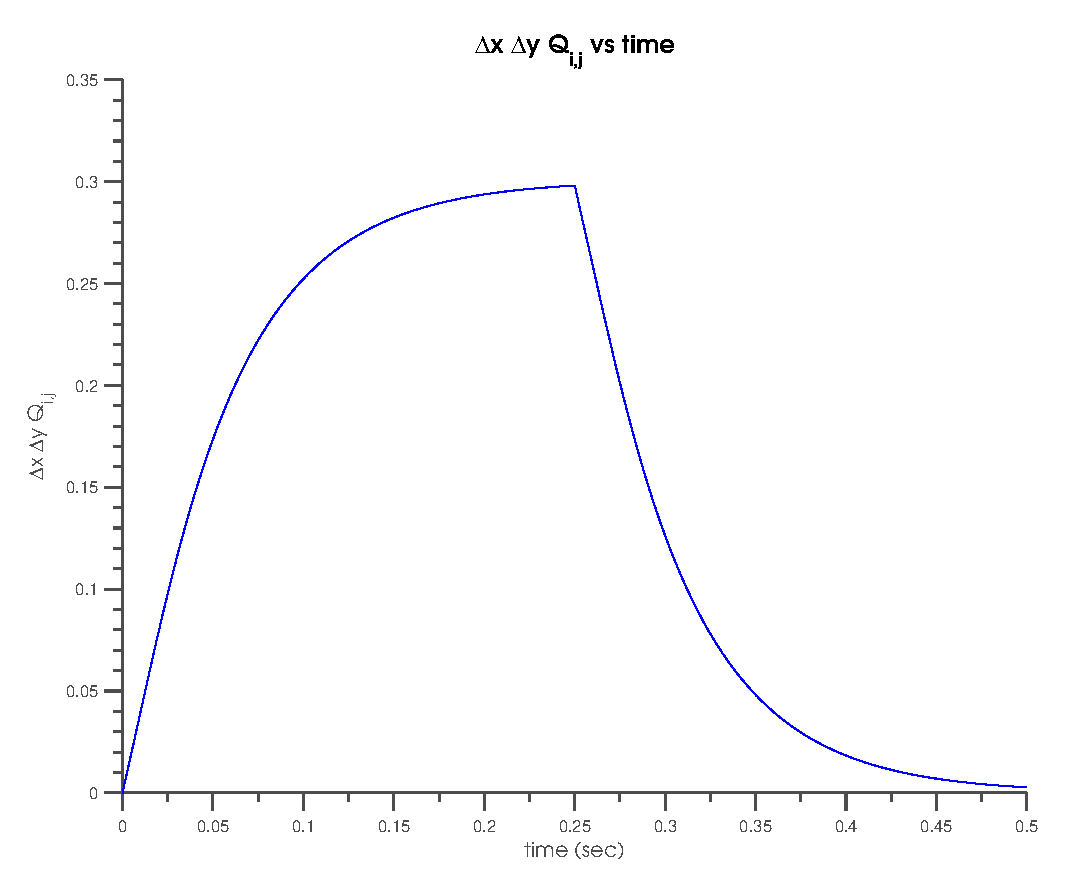
\includegraphics[width=.48\textwidth]{Figures/deltaConservationPlot.eps} \label{fig:deltaConservationPlot}} % (subfigure 1)
	\subfigure[Source - Gaussian Distribution at center]{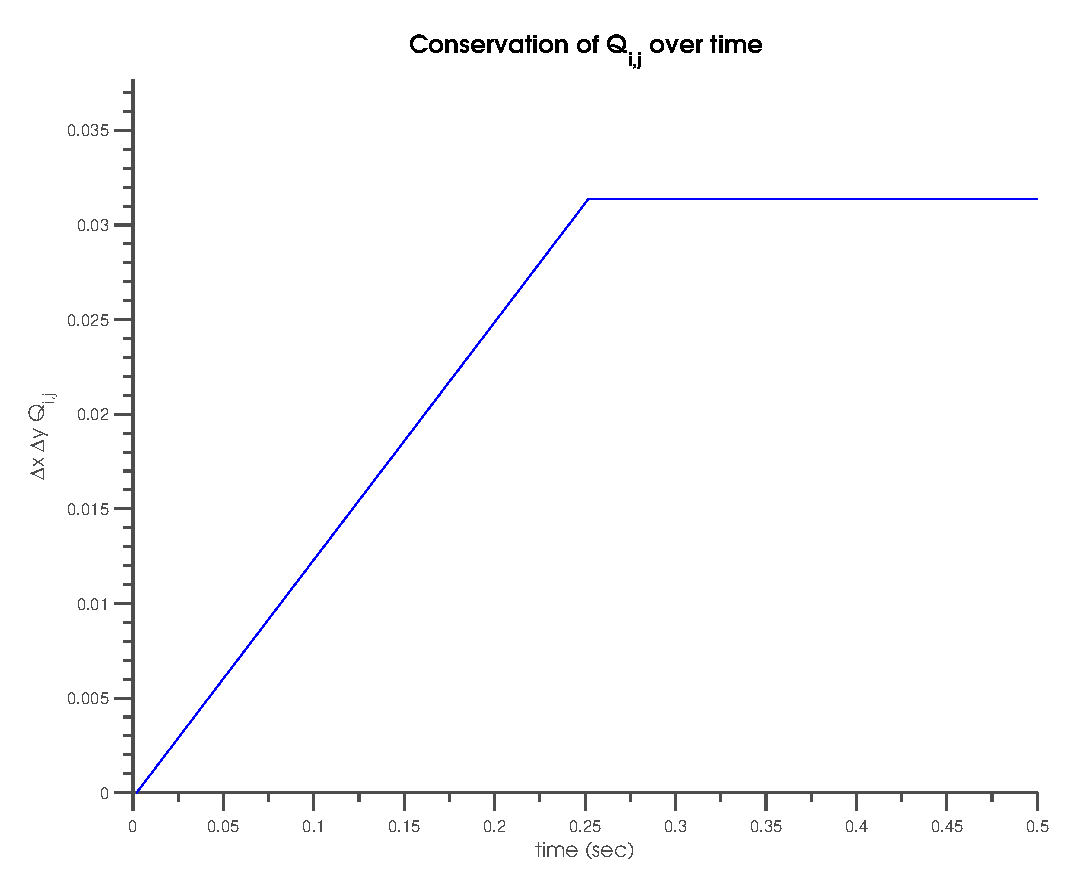
\includegraphics[width=.48\textwidth]{Figures/sourceConservationPlot.eps} \label{fig:sourceConservationPlot}} % (subfigure 2)
	\caption{Plot of Equation~\eqref{eq:numConservation} to show conservation of the quantity $Q_{i,j}$ over time.  The plot has a source term adding heat to the system, but after $t=0.25~s$, the source is shut off and the amount of Q does not change over time.}
\end{figure} % (fig:Figures_fronttrackingfig4)

	\begin{itemize}
		\item[i.] \textbf{Time-discretization and how your code handles the discontinuity in g(t)}
		
		{\color{blue} My code handles the discontinuity in g(t) by using two loops with the first loop including the source term and going from $t=0$ to $t= ts \cdot \tau$ where $ts=\mathrm{round}(0.25/\tau)$.} 
		\item[ii.] \textbf{Space-discretization; where in the cell does (x,y)=(1/2,1/2) appear? different for odd and even m,n}
		
		{\color{blue} The cell (1/2, 1/2) appears only for odd values of m,n and is at $(m+1)/2$. For example, if $m=n=11$, then $(x_{6},y_{6}) = (1/2,1/2)$.} 
	\end{itemize}
\end{enumerate}

% section numerical_results (end)

\newpage
\pagebreak

% This LaTeX was auto-generated from an M-file by MATLAB.
% To make changes, update the M-file and republish this document.

\documentclass{article}
\usepackage{graphicx}
\usepackage{color}

\sloppy
\definecolor{lightgray}{gray}{0.5}
\setlength{\parindent}{0pt}

\begin{document}

    
    
\subsection*{Contents}

\begin{itemize}
\setlength{\itemsep}{-1ex}
   \item Initialize Source function
   \item * Set up the Laplacian operator matrix
   \item * Initialize Q-matrix
   \item * Compute A-matrix (Tn+1)=ATn
   \item * Initialize loop and plot variables
   \item * Loop over desired number of steps
   \item Plot
\end{itemize}
\begin{verbatim}
% heat_equation - Program to solve the diffusion equation
% using the Backward Euler method
clear; help heat_equation; % Clear memory and print header

%* Initialize parameters (time step, grid spacing, etc.)
tau = 1e-4; % Enter time step
N = 100; % Number of grid points
L = 1; % The system extends from (x)=(0) to (x)=(L)
h = L/N;
i = 0:(N-1);
x = h/2 + i*h;
w = 0.2;
xs = 0.5;
ys = 0.5;
\end{verbatim}

        \color{lightgray} \begin{verbatim}  heat_equation - Program to solve the diffusion equation
  using the Backward Euler method

\end{verbatim} \color{black}
    

\subsection*{Initialize Source function}

\begin{verbatim}
S = zeros(N); % Set all elements to zero
xExponent = (x'-xs).^2;
S = exp(-xExponent/w^2);
deltaFunction = zeros(N,1);
deltaFunction(round(N/2))=2;
\end{verbatim}


\subsection*{* Set up the Laplacian operator matrix}

\begin{verbatim}
lap = zeros(N);  % Set all elements to zero
coeff = 1/h^2;
for i=2:(N-1)
    lap(i,i-1) = coeff;
    lap(i,i) = -2*coeff;  % Set interior rows
    lap(i,i+1) = coeff;
end
% Boundary conditions
lap(1,1)=-coeff;
lap(1,2)=coeff;
lap(N,N)=-coeff;
lap(N,N-1)=coeff;
\end{verbatim}


\subsection*{* Initialize Q-matrix}

\begin{verbatim}
Q = deltaFunction;
\end{verbatim}


\subsection*{* Compute A-matrix (Tn+1)=ATn}

\begin{verbatim}
dM = eye(N) - tau*lap;
\end{verbatim}


\subsection*{* Initialize loop and plot variables}

\begin{verbatim}
max_iter = .5/tau;
time = linspace(0,max_iter*tau,max_iter);      % Record time for plots
Qplot(:,1) = Q; % initial value
\end{verbatim}


\subsection*{* Loop over desired number of steps}

\begin{verbatim}
for iter=2:round(.25/tau)
    %* Compute new temperature
    Q = dM\(Q)+deltaFunction;
    Qplot(:,iter) = Q(:);
end
for iter=round(.25/tau):max_iter
    %* Compute new temperature
    Q = dM\(Q);
    Qplot(:,iter) = Q(:);
end
\end{verbatim}


\subsection*{Plot}

\begin{par}
figure(2);clf; mesh(time,x,Qplot); xlabel('t (s)'); ylabel('x (m)'); \%\% Print Plots saveFigurePath = '/Users/kevin/SkyDrive/KTH Work/LaTeX Reports/Heat Equation/Figures/'; \%\% Plot 1 set(figure(2), 'PaperPositionMode', 'auto'); print('-depsc2', [saveFigurePath ...     sprintf('deltaFunctionPlot')]);
\end{par} \vspace{1em}



\end{document}
    

%!TEX root = /Users/kevin/SkyDrive/KTH Work/LaTeX Reports/Heat Equation/Heat Equation.tex

% This LaTeX was auto-generated from an M-file by MATLAB.
% To make changes, update the M-file and republish this document.



 
    
\section*{2-D Matlab Code}

\begin{itemize}
\setlength{\itemsep}{-1ex}
   \item * Set up the Laplacian Matrix x-direction
   \item * Combine lap with identity matrix
   \item Initialize Source function
   \item * Initialize loop and plot variables
   \item * Loop over desired number of steps (wave circles system once)
   \item Plot
\end{itemize}
\begin{verbatim}
% TwoDHeatEquation - Program to solve the diffusion equation
% using the Backward Euler method
clear; help TwoDHeatEquation; % Clear memory and print header

%* Initialize parameters (time step, grid spacing, etc.)
tau = 0.05; % Enter time step
N = 100; % Number of grid points
L = 1; % The system extends from (x,y)=(0,0) to (x,y)=(L,L)
h = L/N;
i = 0:(N-1);
j = 0:(N-1);
x = h/2 + i*h;
y = h/2 + j*h;
w = 0.2;
xs = 0.5;
ys = 0.5;
\end{verbatim}

        \color{lightgray} \begin{verbatim}  TwoDHeatEquation - Program to solve the diffusion equation
  using the Backward Euler method

\end{verbatim} 
\color{black}
    

\subsection*{* Set up the Laplacian Matrix x-direction}

\begin{verbatim}
lap = zeros(N);  % Set all elements to zero
coeff = 1/h^2;
for i=2:(N-1)
    for j=2:(N-1)
        lap(i,i-1,j) = coeff;
        lap(i,i,j) = -4*coeff;  % Set interior rows
        lap(i,i+1,j) = coeff;
        lap(i,i,j-1) = coeff;
        lap(i,i,j+1) = coeff;
    end
end
lap(1,1,1)=-coeff;
lap(1,2,2)=coeff;
lap(N,N,N)=-coeff;
lap(N,N-1,N-1)=coeff;
iMatrix=zeros(N,N,N);
iMatrix(1:1+N+N^2:end)=1;
\end{verbatim}


\subsection*{* Combine lap with identity matrix}

\begin{verbatim}
dM = iMatrix - tau*lap;
\end{verbatim}


\subsection*{Initialize Source function}

\begin{verbatim}
S = zeros(N); % Set all elements to zero
xExponent = (x'-xs).^2;
yExponent = (y-ys).^2;
S = exp(-xExponent/w^2);
Q0 = S;
S3D = exp(-xExponent/w^2)*exp(-yExponent/w^2);
mesh(S3D);
\end{verbatim}

\subsection*{* Initialize loop and plot variables}

\begin{verbatim}
max_iter = .5/tau;
time = linspace(0,max_iter*tau,max_iter);
Qplot(:,1) = S; % initial value set to source
\end{verbatim}


\subsection*{* Loop }

\begin{verbatim}
for iter=2:round(.25/tau)
    %* Compute new temperature
    Q0 = dM\(Q0)+S;
    Qplot(:,iter) = Q0(:);
end
for iter=round(.25/tau):max_iter
    %* Compute new temperature
    Q0 = dM\(Q0);
    Qplot(:,iter) = Q0(:);
end
\end{verbatim}

        \color{lightgray} \begin{verbatim}Error using \
Inputs must be 2-D, or at least one input must be scalar.
To compute elementwise LDIVIDE, use LDIVIDE (.\) instead.

Error in TwoDHeatEquation (line 54)
    Q0 = dM\(Q0)+S;
\end{verbatim} 
\color{black}
    

\subsection*{Plot}

\begin{verbatim}
figure(2);clf;
mesh(time(length(time)/2:end),x,Qplot(:,length(time)/2:end));
xlabel('t'); ylabel('x');
\end{verbatim}



    

\bibliographystyle{IEEEtran}
\bibliography{HeatEquation}
%\noindent Updated \today.} 
\end{document} 
